% Chapter Template

\chapter{Dataset} % Main chapter title

\label{ch:04} % Change X to a consecutive number; for referencing this chapter elsewhere, use \ref{ChapterX}

%----------------------------------------------------------------------------------------
%	SECTION 1
%----------------------------------------------------------------------------------------

 In this thesis, we require two kinds of input data to train our models. 
First, we need to know the geometry of the object surface. This can be collected by a depth camera, which records the Z-axis distance of the object surface to the camera position and it can be further converted to a point cloud. 
Second, we need illuminated information of the object surface, which considers a photometric-information used for further improvement. 
This kind of information requires an observed image of the object with the light directions projected onto the object surface. 

In order to gain these data, we can use a light scanner to scan the objects in the laboratory. However, the scanner usually can not scan the dark, shiny, and transparent regions, which leaves plenty of missing pixels and holes in the depth map. This incomplete surface information raises the difficulty for our model training since the ground-truth corresponding to the depth map will be incomplete as well. Second, training a deep learning-based model usually requires a huge dataset, especially for a network without a backbone. To create a single depth map dataset for this thesis would be too much work and resource requirements. A proper way for getting huge depth map data with illumination information can be considered using a game engine, which can simulate any number of data that we require.

In this thesis, we use the Unity game engine for data generation. By using a $ C\# $ script, we can set up a similar configuration in the laboratory. Then create a mount of data based on the collected objects. The dataset that we created for this thesis is called \textit{synthetic-50-5} since it has 50 different object models for training and 5 object models for testing.



\section{Resource}
The object model we used are searched from internet.
A set of point cloud datasets for computer vision research has been published by /cite[data1], /cite[data2], /cite[data3] and /cite[data4]. These point clouds are scanned from real objects using high resolution scanners like Cyberware 3030 MS+ and calibrated with post processing. All objects has been scanned for hundreds of times with an exhaustive completion for the origin objects, which is up to millions points. (\cite{data1}). The dense point clouds make the normal inference task trivial since the neighbor based method performs adequately for this kind of task. Some of the point clouds even contain pre-computed normal maps based on more advanced methods. They all provide the accurate ground truth for the supervised learning method.

The \textit{synthetic50-5} is a dataset we generated in this thesis based on 50 point clouds as a training set and 5 point clouds as a test set. When we create the dataset, we tried to make the object types as many as possible to give a robust and wide range covered training scenarios. There are various categories of models, such as figure, animal, statue, toy, furniture, antique, and car model, some of which have relatively smooth surfaces, such as /textit[arm, bus, bunny, cat, zebra], and some of which have highly complicated details, such as \textit{Washington, Car-Engine, Armadillo}. 
We created this dataset for normal inference tasks. Figure \ref{fig:dataset-demo} gives the illustrations of some objects. Appendix \ref{AppendixA} gives a full version of dataset models.

\begin{figure}[!h]
	\centering
	\begin{subfigure}[b]{0.24\linewidth}
		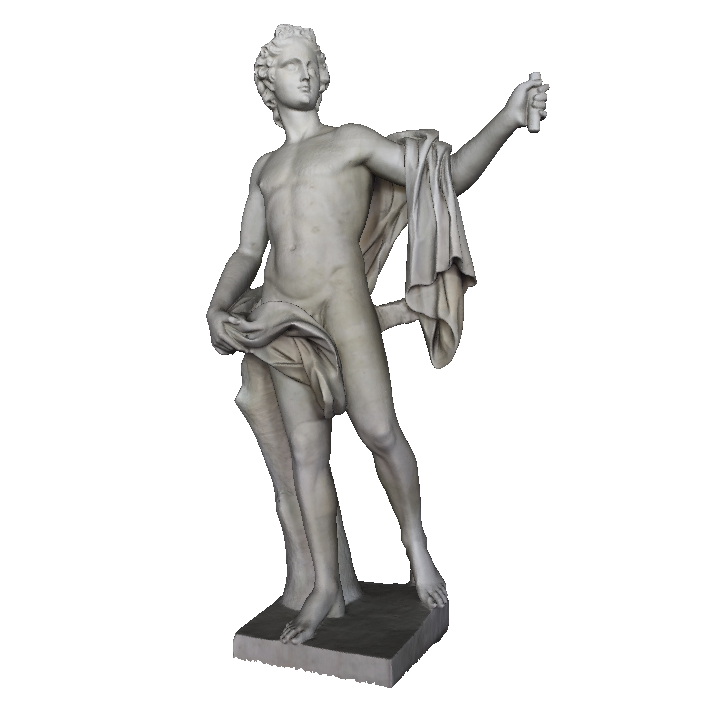
\includegraphics[width=\linewidth]{./Figures/train-dataset/00.apoll.png}
		\caption{apoll}
	\end{subfigure}
	\begin{subfigure}[b]{0.24\linewidth}
		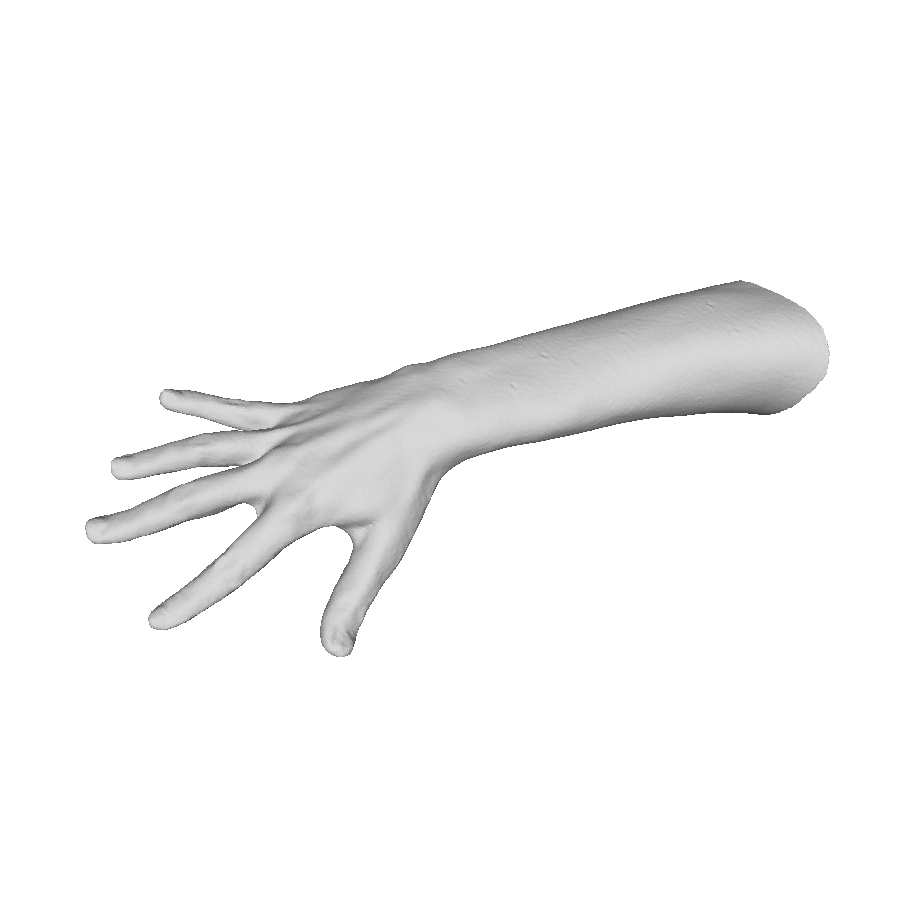
\includegraphics[width=\linewidth]{./Figures/train-dataset/01.arm.png}
		\caption{arm}
	\end{subfigure}
	\begin{subfigure}[b]{0.24\linewidth}
		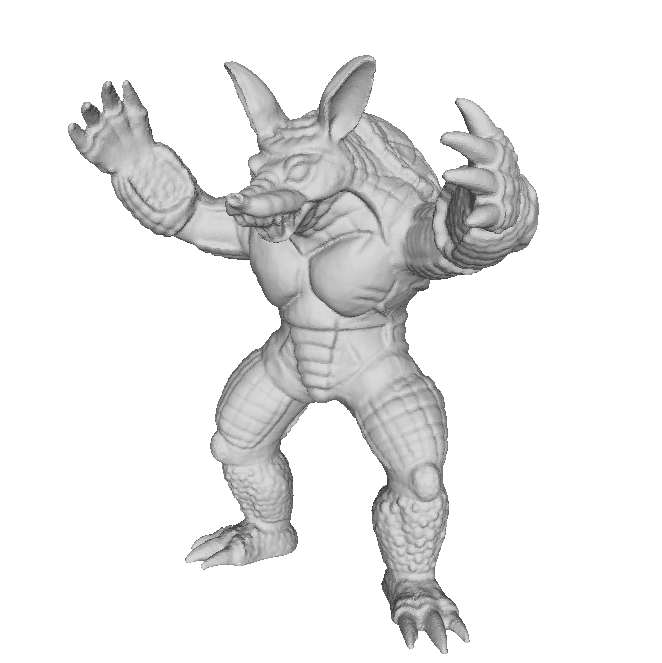
\includegraphics[width=\linewidth]{./Figures/train-dataset/02.armadillo.png}
		\caption{armadillo}
	\end{subfigure}
	\begin{subfigure}[b]{0.24\linewidth}
		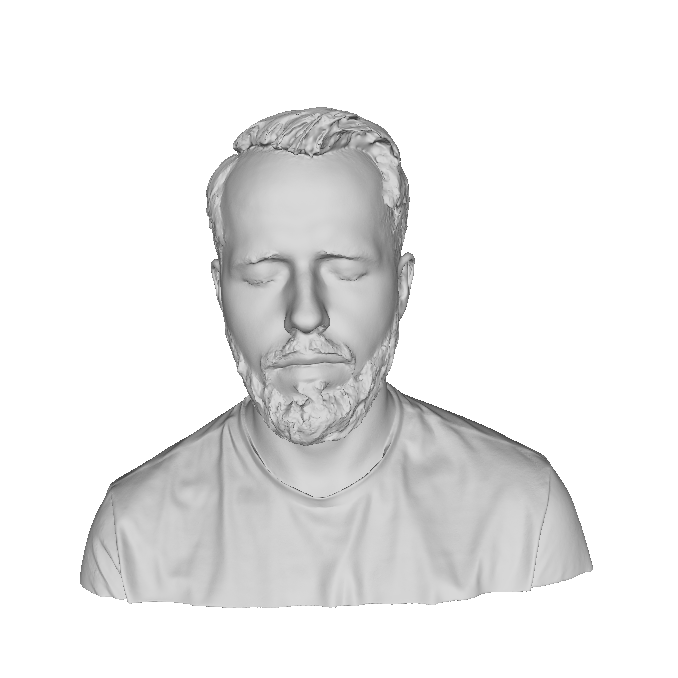
\includegraphics[width=\linewidth]{./Figures/train-dataset/03.bearded-guy.png}
		\caption{bearded-guy}
	\end{subfigure}
	
	\begin{subfigure}[b]{0.24\linewidth}
		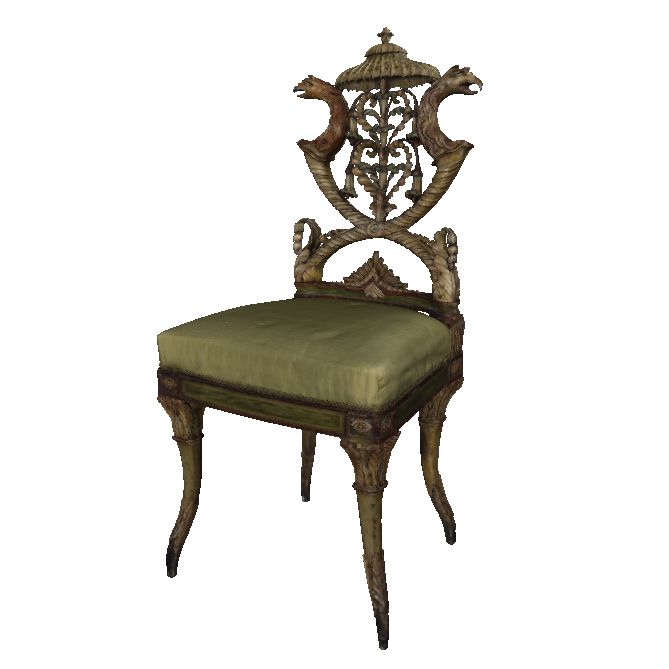
\includegraphics[width=\linewidth]{./Figures/train-dataset/08.pergolesi-side-chair_texture.png}
		\caption{chair}
	\end{subfigure}
	\begin{subfigure}[b]{0.24\linewidth}
		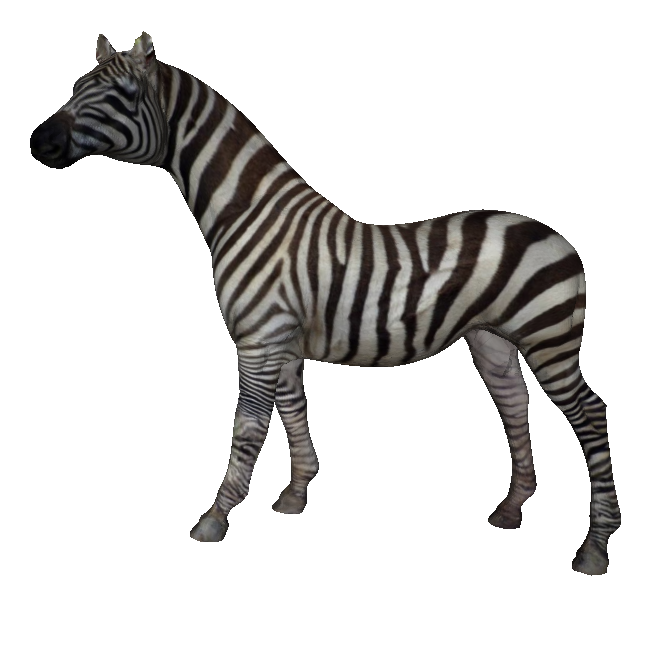
\includegraphics[width=\linewidth]{./Figures/train-dataset/42.zebra_texture.png}
		\caption{zebra}
	\end{subfigure}
	\begin{subfigure}[b]{0.24\linewidth}
		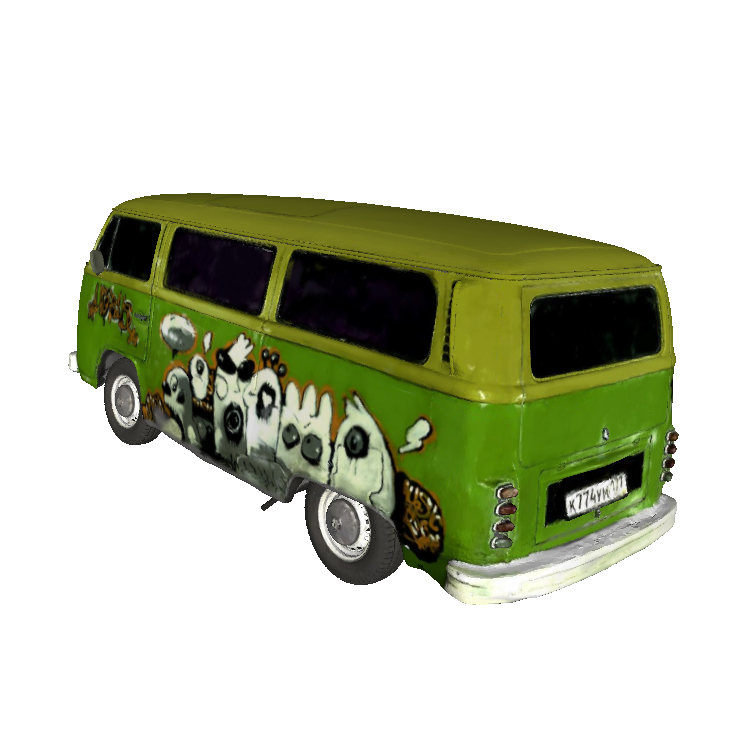
\includegraphics[width=\linewidth]{./Figures/test-dataset/01.bus_texture.png}
		\caption{bus}
	\end{subfigure}
	\begin{subfigure}[b]{0.24\linewidth}
		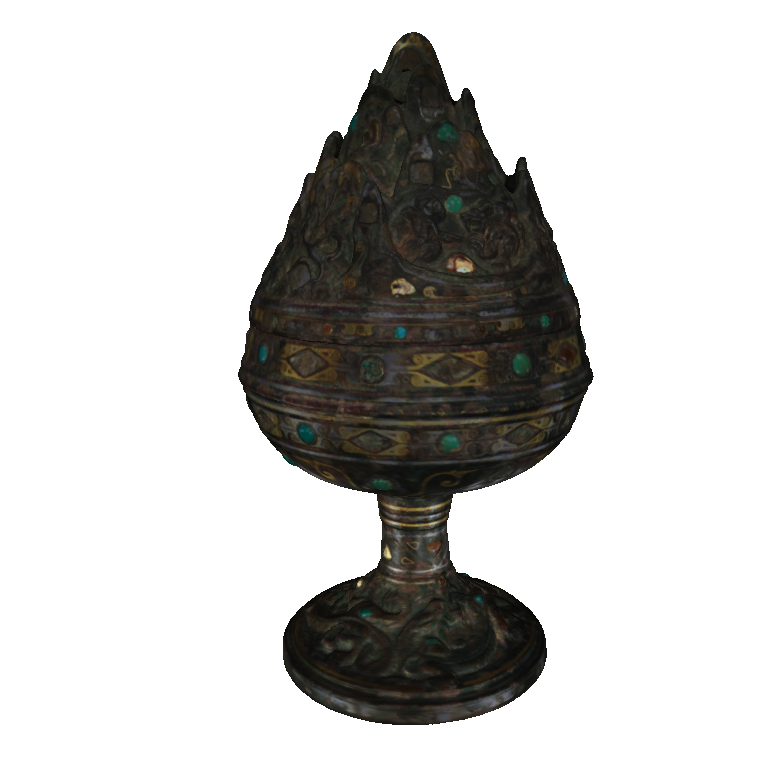
\includegraphics[width=\linewidth]{./Figures/test-dataset/03.baoshanlu_texture.png}
		\caption{baoshanlu}
	\end{subfigure}
	\decoRule
	\label{fig:dataset-demo}
	\caption{Point clouds scanned by high resolution scanners}
\end{figure}
Besides, some objects also have colored textures, as shown in the second row of Figure \ref{fig:dataset-demo}. This is specially prepared for the illuminated approach since they will take the image into account to evaluate the surface normal. By using textured models, our models become closer to the real dataset and have improved robustness, which can apply to the real dataset further.



\definecolor{direction-light-color}{RGB}{255,244,214}
\newcommand{\col}[1]{%
	\textcolor{#1}{\vrule width 0.5cm}}
\section{Synthesize Scenes using Unity}
In order to simulate the data collection scenario close to the real world as much as possible. We did the following settings. A flat cylinder called $ stage $ is placed in the center of the 3D space as a platform to place objects. We fixed the stage in a predetermined position, which is not changed when images are captured. 
To provide ambient light, one directional light with RGB color FFF4D6 /col[direction-light-color] is placed in a top-view direction at a distance of 25 meters, which also has a fixed location.
An RGB-D camera is placed in a top-view direction around 10m away from the stage. The camera captures the depth map and the gray-scale image, which is randomly arranged after each scene. The moving range of the camera has 0.1m in both directions of the X, Y, and Z axis and a 1-degree random changed Euler angle. 
As an illumination light, a point light is placed around 5 meters away, which is also randomly moved after each scene. The moving range is 0.3m in both directions of the X, Y, and Z axis and 1 degree random in the Euler angle.

During the data collection, the object is randomly selected and placed on the stage. The object has a random up to 30 degrees rotation align $ roll $-axis, 30-degrees rotation aligns $ pitch $-axis, and 180-degrees rotation aligns $ yaw $-axis. Thus the camera has the opportunity to capture every direction of the object and consequently abundant the dataset. The layout in the Unity game engine is shown in Figure \ref{fig:unity-workplace}. We generate 3000 scenes with resolution $ 128\times128 $ and 5000 scenes with resolution $ 512\times512 $.

\begin{figure}[h!]
	\centering
	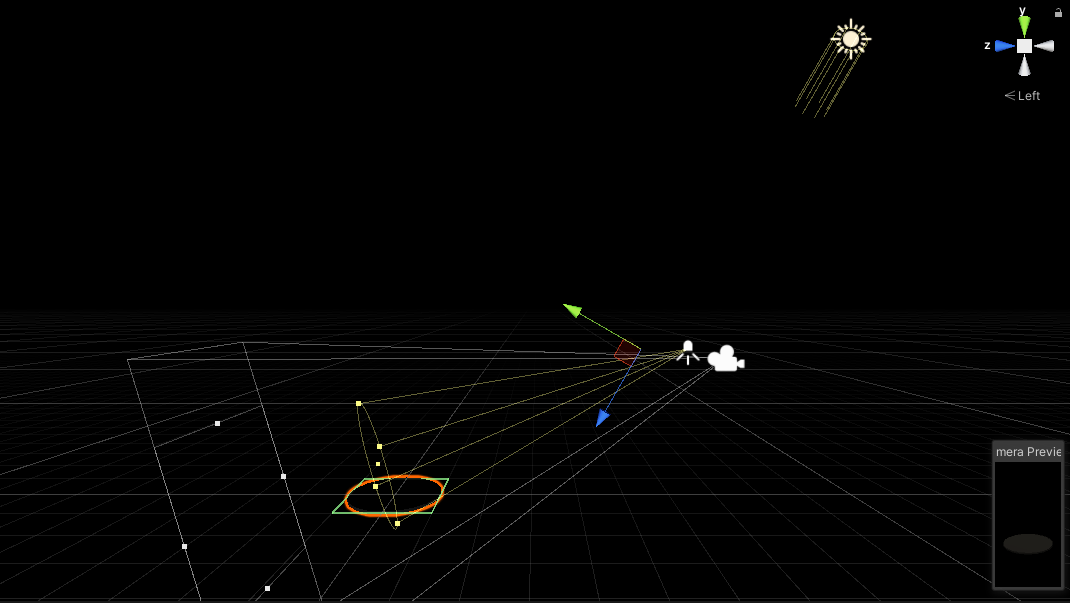
\includegraphics[width=.99\textwidth]{./Figures/unity-workplace.PNG}
	\decoRule
	\caption{The layout of synthetic scenes generation in Unity.}
	\label{fig:unity-workplace}
\end{figure}
The main advantage of generated scenes is the availability of complete information. We can capture the depth map in a lossless way. The corresponding normal map can also be safely considered as ground truth. And the scale of the dataset is easy to control. Table \ref{tab:data-files} gives more dataset information.
\begin{table}
	\caption{The information saved for each scene in ``synthetic50-5".}
	\label{tab:data-files}
	\centering
	\begin{tabular}{l l}
		\toprule
		\tabhead{Data} & \tabhead{Size} \\
		\midrule
		Depth map & Width$ \times $Height$ \times $ 1 \\
		\hline 
		Depth range  & MinDepth, MaxDepth \\  
		\hline
		Grayscale Image	&  Width$ \times $Height$ \times $ 1 \\  
		\hline 
		Normal Map &   Width$ \times $Height$ \times $ 3  \\
		\hline 
		Light Position &  $ 3\times1 $  \\
		\hline
		Camera Intrinsic Matrix &  $ 3\times 3 $  \\
		\hline 
		Camera Extrinsic Matrix &  $ 3\times 4 $  \\
		\hline 
		\bottomrule
	\end{tabular}
\end{table}

One critical detail that we must care about is camera exposure. Or we have to control the light radiance on the object surface. As shown in figure \ref{fig:camera_exposure}, too little exposure will neutralize the illumination information, resulting in an ambient light effect. Too much exposure makes the surface texture hard to recognize. When we did the experiments, we found that a suitable light setting is essential to the illumination-based approach. Too much or too few light effects won't improve the illumination-based approach.

\begin{figure}[H]
	\centering
	\begin{subfigure}[b]{0.32\linewidth}
		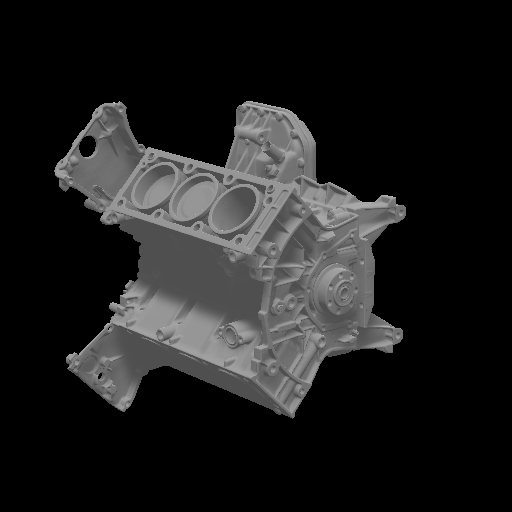
\includegraphics[width=\textwidth]{./Figures/wrong_exposure_2.png}
		\caption{Too dim}
	\end{subfigure}
	\begin{subfigure}[b]{0.32\linewidth}
		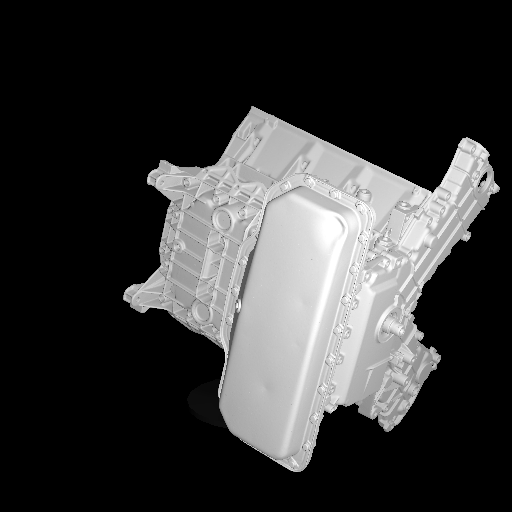
\includegraphics[width=\textwidth]{./Figures/right_exposure.png}
		\caption{Just Right}
	\end{subfigure}
	\begin{subfigure}[b]{0.32\linewidth}
		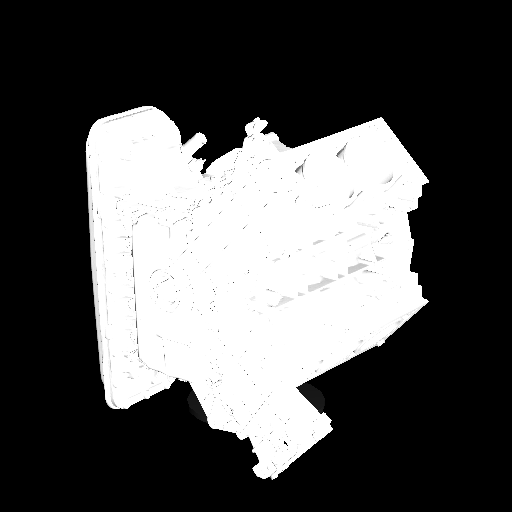
\includegraphics[width=\textwidth]{./Figures/wrong_exposure.png}
		\caption{Too bright}
	\end{subfigure}
	\decoRule
	\caption{Different exposure to the objects.}
	\label{fig:camera_exposure}
\end{figure}




\section{Data preprocessing}
The raw data captured from Unity required further preprocessing before feeding them into the training models. 
A depth map is captured by a depth camera in Unity, which is a 1 channel image that contains information relating to the distance of the surfaces of the scene objects from a viewpoint. It can be saved as a 16-bit gray-scale image, i.e. each pixel in the range $0 - 65535$. 


The gray-scale image can be used as a guided normal inference task and also as a readable scene for humans. Since the image captured by the camera is in RGB format, we need to convert it to gray colors for our models. It is based on the following equation.
\[ gray: \frac{R+2G+B}{4}  \]

The normal map is the tangent surface normal, which is saved in a 32-bit RGB color image. The surface normal $ (n_x, n_y, n_z) $ and its corresponding RGB color $ (R,G,B) $ can be converted based on the following equation:
\begin{dgroup*}
	\begin{dmath*}
		n_x = \frac{R}{255} * 2 - 1
	\end{dmath*}
	\begin{dmath*}
		n_y = \frac{G}{255}*2 - 1
	\end{dmath*} 
	\begin{dmath*}
		n_z = 1-\frac{B}{255} * 2
	\end{dmath*}
\end{dgroup*}

If consider the relation between Lambertian reflection and normal direction, the light source can be used to calculate the reflect direction of each point.

The camera intrinsic and extrinsic matrix helps point cloud calculation.

\subsection{Convert to Point Cloud}
\label{sec:depth-map-to-point-cloud}

The depth map can be converted to a 3D vertex point cloud as the input of the normal inference model. 

\begin{figure}[h!]
	\centering
	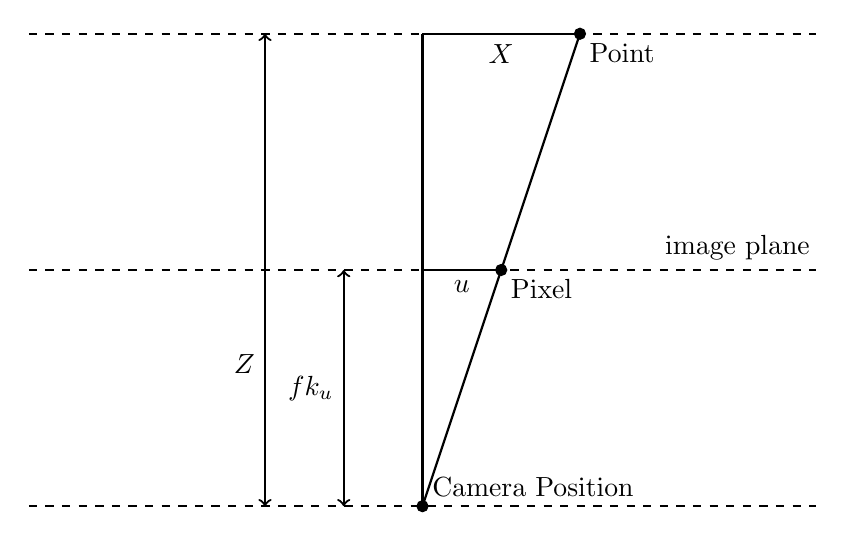
\begin{tikzpicture} 
		% reference lines
		\draw[thick,dashed]	(0,0) -- (10,0) ; % bottom
		\draw[thick,dashed]	(0,3) -- (10,3) node[pos=0.9, above] {image plane}; % middle
		\draw[thick,dashed]	(0,6) -- (10,6); % top
		% camera 
		\filldraw[black] (5,0) circle (2pt) node[anchor=south west]{Camera Position};
		% world point 
		\filldraw[black] (7,6) circle (2pt) node[anchor=north west]{Point};
		% image point
		\filldraw[black] (6,3) circle (2pt) node[anchor=north west]{Pixel};
		% similiar triangles
		\draw[thick] (5,0) -- (5,6); % AB
		\draw[thick] (5,0) -- (7,6); % AC
		\draw[thick] (5,6) -- (7,6) node[midway, below] {$ X $}; % BC
		\draw[thick] (5,3) -- (6,3) node[midway, below] {$ u $};
		% measure arrows
		\draw[thick, <->] (4,0) -- (4,3) node[midway, left] {$ fk_u $};
		\draw[thick, <->] (3,0) -- (3,6) node[pos=0.3, left] {$ Z $};
	\end{tikzpicture}	
	\decoRule
	\caption{Convert depth to point in camera coordinate system}
	\label{fig:depth-triangulation}
\end{figure}

Consider a 3-dimensional Euclidean space. Use $ z $ axis to denote the depth. The $ x  $ and $ y $ axis are perpendicular to each other. For a pixel $ (u,v) $ on depth map, its depth $ D(u,v) $ is the $ Z $ component of the corresponding point $P_C = (X,Y,Z) $ regarding camera coordinate system. The $ X $ and $ Y $ can be calculated based on the triangle similarity.
\begin{dgroup*}
	
	\begin{dmath*}
		X = \frac{uZ}{fk_u}
	\end{dmath*}
	\begin{dmath*}
		Y = \frac{vZ}{fk_v}
	\end{dmath*}
\end{dgroup*}
where $ fk_u, fk_v $ is the focal length in pixels align $ u $ and $ v $ axes.
Converted a point from camera coordinate system to the world coordinate system, using extrinsic matrix $ R $ and $ t $
\[P_W = P_CR+t \]

\subsection{Point Cloud Normalization}
\label{sec:dataset-normalization}
%% How to represent input tensor, to make it fast converse
The sizes of each training object are various, whereas it should be as an invariant value for the training model. Thus normalization is required before feeding training objects into the models.
We showed the data fluctuation in each axis in Figure \ref{fig:data-range}. Table \ref{tab:data-range} gives a quantitative evaluation of the corresponding average values. 

The normalization has been performed as follows. First, translate the points to the original point as close as possible, then choose the range value of one axis as a scale factor, and normalize the points to unit vectors. The equation is shown as follows
\begin{dgroup*}
	
	\begin{dmath*}
		X_n =\frac{X-\min(X)}{s}
	\end{dmath*}
	\begin{dmath*}
		Y_n = \frac{Y-\min(Y)}{s}
	\end{dmath*}
	
	\begin{dmath*}
		Z_n = \frac{Z-\min(Z)}{s}
	\end{dmath*}
\end{dgroup*}

where $ s $ is a scale factor, 

\begin{dmath*}
	s = \max(X)-\min(X)
\end{dmath*}
It is calculated as the range of the $ X $ axis, but theoretically can be used by the $ Y $ or $ Z $ axes as well.

\begin{figure}[!h]
	\centering
	{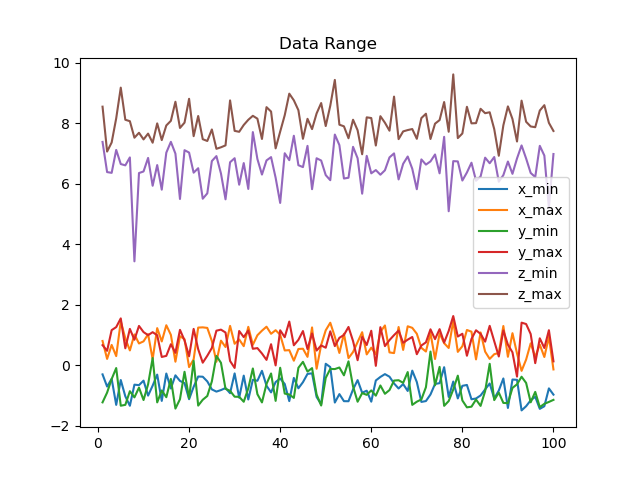
\includegraphics[width=0.45\textwidth]{./Figures/Data_Extreme.png}}
	{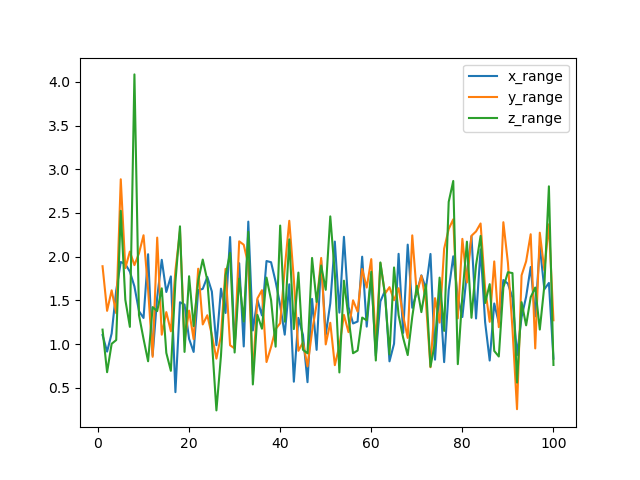
\includegraphics[width=0.45\textwidth]{./Figures/Data_Range.png}}
	\label{fig:data_range}
	\decoRule
	\caption{Left: Extreme value in 3 axis; Right: Vertex range in 3 axis}
\end{figure}

\begin{table}[th]
	\label{tab:data-range}
	\centering
	\begin{tabular}{c | c c c}
		\toprule
		\tabhead{Axis} & \tabhead{Scale} & \tabhead{Min} & \tabhead{Max}\\
		\midrule
		X & 1.48 & -0.75 & 0.73\\
		\hline 
		Y & 1.56 & -0.76 & 0.80\\
		\hline 
		Z & 1.47 & 6.53 & 8.00\\
		\bottomrule
		
	\end{tabular}
	\caption{ The fluctuation of extreme values and their ranges in 100 random training items. }
\end{table}



\subsection{Noise}
\label{sec:noise}
The raw depth maps captured by light scanners usually have missing pixels. In order to fit well with real data, the synthetic data has been added uniform distributed noise, which randomly removes the valid pixels in the maps.
The simulated noise is distributed evenly around the whole map with specific noise intensity. A parameter $ \mu $ is used to control the intensity of noise. It denotes the $ \mu $-percent pixel drop-off. For example, $ \mu-10 $ removes 10\% pixels randomly. For each scene, the noise operation based on a random $ \mu $ in a range $ \left[0, 50\right]  $ is used. Some scenes have more missing pixels and some have fewer. The random noise intensity also enables the model to learn scenarios not only with noise but also with minor noise or even without noise.
Figure \ref{fig:noise-intensity} shows the noise effect with different $ \mu $.
%% add noise image
\begin{figure}[!h]
	\centering
	{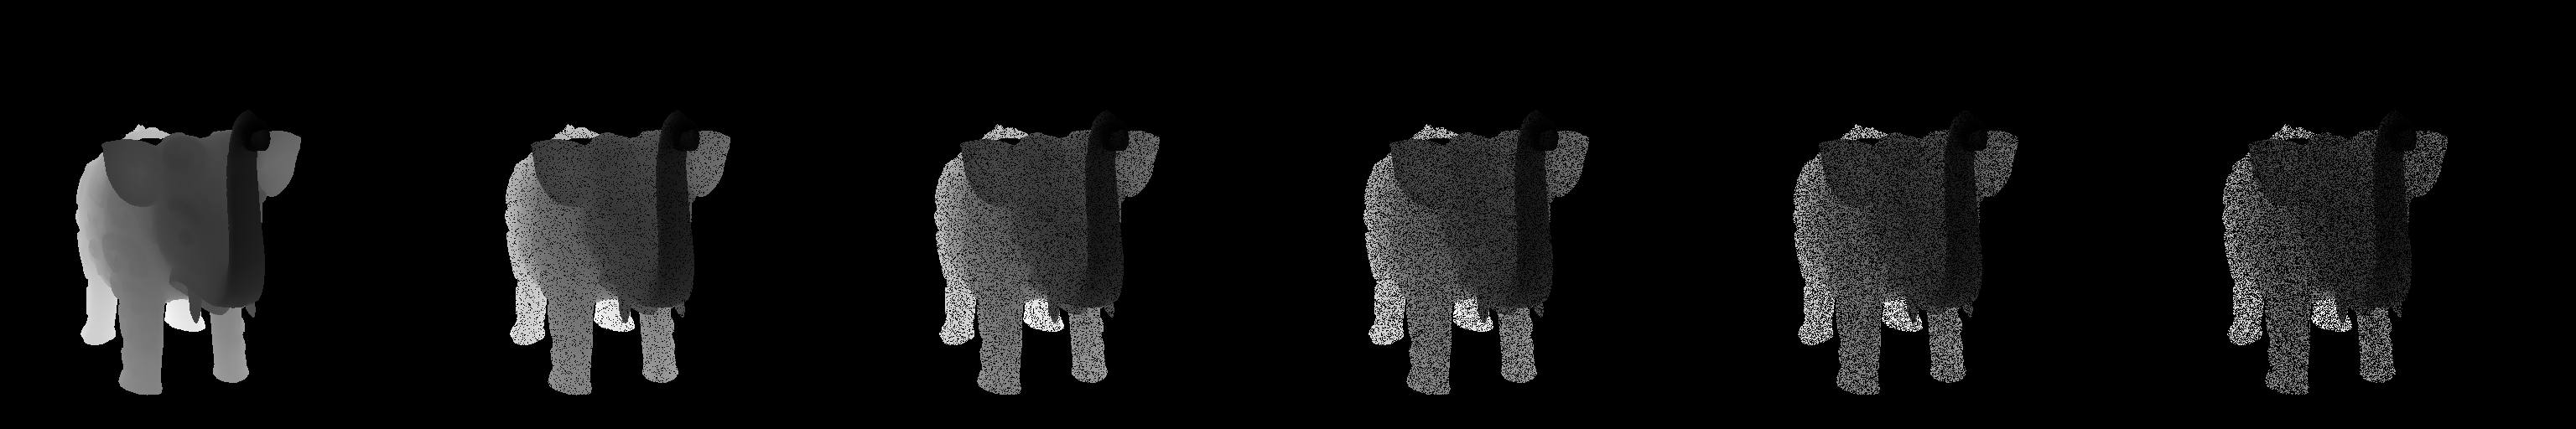
\includegraphics[width=.9\textwidth]{./Figures/add_noise_depth.png}}
	\decoRule
	\caption{Noise-intensity on $ \mu-0, \mu-10,\mu-20, \mu-30, \mu-40, \mu-50,$. Object Name: elephant-zun-lid.}
	\label{fig:noise-intensity}
\end{figure}


\subsection{Fit to PyTorch}
In order to save training time, we compress the dataset in PyTorch format. The structure of a single item is shown in Table \ref{tab:tensor-structure}.
\begin{table}[H]
	\caption{The structure of a single tensor in the dataset.}
	\label{tab:tensor-structure}
	\centering
	\begin{tabular}{l | l}
		\toprule
		\tabhead{Name} & \tabhead{Content} \\
		\midrule
		\multirow{3}{*}{input-tensor}  & Vertex \\  & Image \\  & Light Direction \\
		\hline
		\multirow{3}{*}{output-tensor}  & GT-Normal \\ & Image \\ & GT-Light-Direction \\
		\hline
		Light position & light position \\
		\hline 
		Camera Matrix  & K,R,t\\
		\hline 
		Depth Range  & minDepth, maxDepth\\
		\bottomrule
	\end{tabular}
\end{table}
